\documentclass[report.tex]{subfiles}
\graphicspath{ \subfix{./images/} \subfix{./graphs/} }
\begin{document}
\section{Milestone 5: Handle settings}

I designed a JSON schema to store the settings in a file in the design section, but after looking through some documentation, I found a better way of storing settings on Windows. I can use local app data store\cite{microsoft:docs:store-and-retrieve-app-data} to store the settings. Compared to storing the settings in JSON, this brings several advantages: the lifecycle of the settings files are managed by Windows, so when the app gets uninstalled, there will not be garbage settings file flying around the user's disk; the user also can't mess around the settings file directly, which reduces the risk of invalid settings; the data is stored in binary instead of plain text file, which saves disk space. Considering all these benefits, I decide to use \code{LocalSettings} container to store the settings.

\subsection{Theme settings}

The colour theme of the app needs to be loaded when the app starts. So in App.xaml.cs, I added logic to handle this in \code{OnLaunched}.

\begin{minted}{csharp}
protected override async void OnLaunched(LaunchActivatedEventArgs args)
{
    // ...
    InitializeTheme();
}

private static void InitializeTheme()
{
    // Load theme
    ApplicationDataContainer localSettings = ApplicationData.Current.LocalSettings;
    var CurrentThemeValue = localSettings.Values["Theme"];

    // if there exists a theme setting, use the theme setting
    // otherwise set the default theme and save it to the setting
    ElementTheme theme;
    if (CurrentThemeValue != null)
    {
        theme = (ElementTheme)CurrentThemeValue;
    }
    else
    {
        theme = ElementTheme.Default;
        localSettings.Values["Theme"] = (int)theme;
    }

    // Apply theme to rootElement
    if (m_window.Content is FrameworkElement rootElement)
    {
        rootElement.RequestedTheme = theme;
    }
}
\end{minted}

In SettingsPage, I need to initialize the current theme on load and save the selected theme to the setting when the checkboxes are checked.

\begin{minted}{csharp}
public SettingsPage()
{
    InitializeComponent();
    // Init theme settings on load
    GetCurrentTheme();
    // ...
}

/// <summary>
/// Get the current theme and set the check box
/// </summary>
private void GetCurrentTheme()
{
    if (App.m_window.Content is FrameworkElement rootElement)
    {
        string currentTheme = rootElement.RequestedTheme.ToString();
        ThemePanel
            .Children
            .Cast<RadioButton>()
            .FirstOrDefault(c => c?.Tag?.ToString() == currentTheme)
            .IsChecked = true;
    }
}

/// <summary>
/// Change the application request theme to the selected theme when the radio button is clicked
/// Save the theme into settings
/// </summary>
/// <param name="sender"></param>
/// <param name="e"></param>
private void ThemeRadioButton_Checked(object sender, RoutedEventArgs e)
{
    var selectedTheme = ((RadioButton)sender)?.Tag?.ToString();

    if (selectedTheme != null && App.m_window.Content is FrameworkElement rootElement)
    {
        rootElement.RequestedTheme = GetEnum<ElementTheme>(selectedTheme);
        ApplicationDataContainer localSettings = ApplicationData.Current.LocalSettings;
        localSettings.Values["Theme"] = (int)rootElement.RequestedTheme;
    }
}
\end{minted}

When I navigate to the settings page, the check box is checked on the current theme correctly.

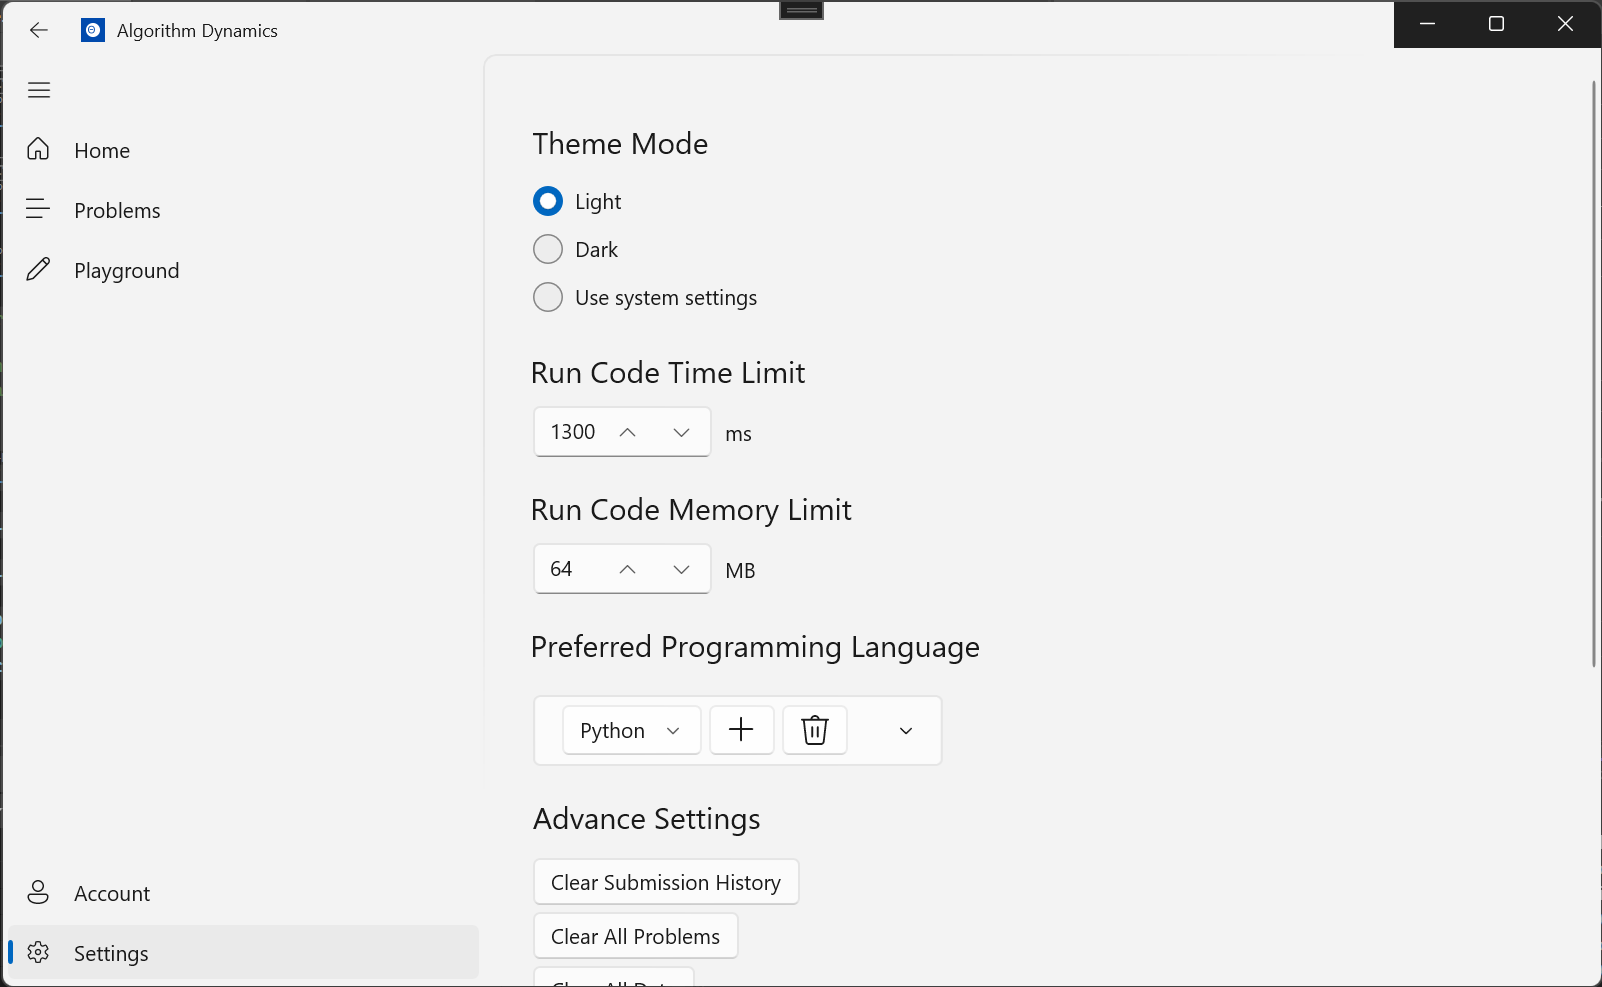
\includegraphics[width=\textwidth, height=\textheight, keepaspectratio]{SettingsPage-InitTheme}

After I change the setting and relaunch the app, the setting is saved correctly.

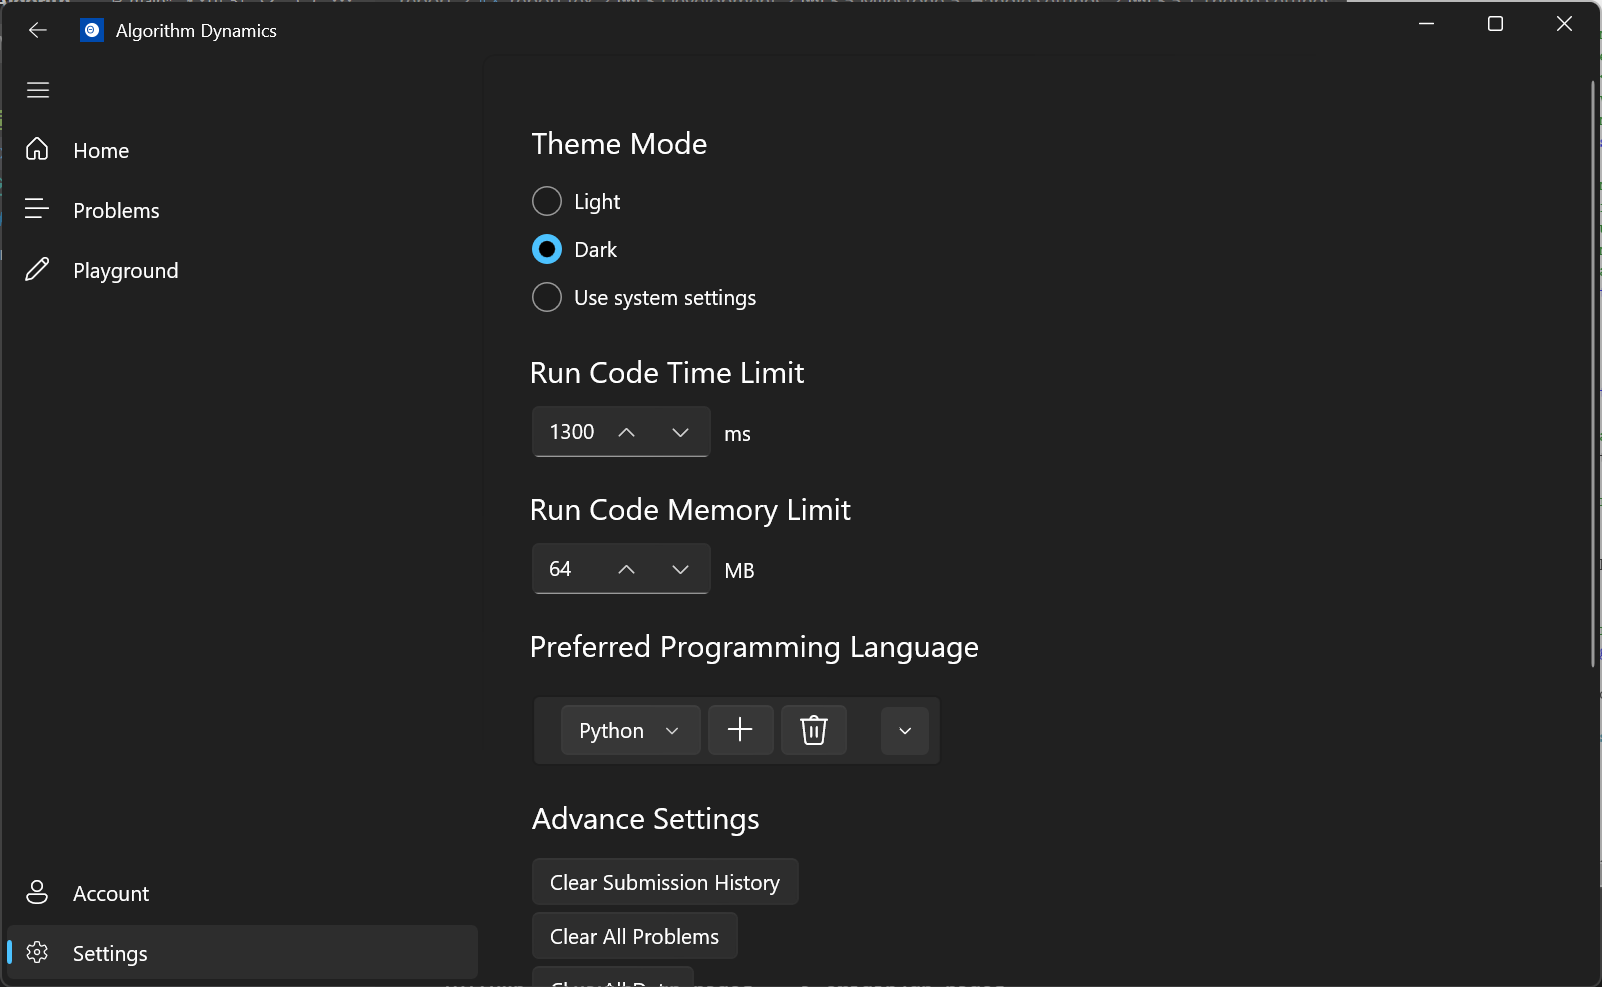
\includegraphics[width=\textwidth, height=\textheight, keepaspectratio]{SettingsPage-SaveTheme}

\subsection{TimeLimit settings}

In the SettingsPage, I add a public attribute \code{TimeLimit}, its setter and getter reads and saves its value directly to the local setting container. After the user input the number, it is first validated by the number box control, then it gets saved directly to the setting, which makes the user experience seamless.

\begin{minted}{csharp}
/// <summary>
/// The RunCode TimeLimit value
/// </summary>
public int TimeLimit
{
    get
    {
        // Read time limit from settings
        // If does not exist, store the default time limit
        ApplicationDataContainer localSettings = ApplicationData.Current.LocalSettings;
        var CurrentValue = localSettings.Values[TIMELIMIT_KEY];
        if (CurrentValue != null)
        {
            return (int)CurrentValue;
        }
        else
        {
            localSettings.Values[TIMELIMIT_KEY] = DEFAULT_RUN_CODE_TIMELIMIT;
            return DEFAULT_RUN_CODE_TIMELIMIT;
        }
    }
    set
    {
        // Update the setting
        ApplicationDataContainer localSettings = ApplicationData.Current.LocalSettings;
        localSettings.Values[TIMELIMIT_KEY] = value;
    }
}
\end{minted}

If invalid input is received, it is automatically rejected and the value is unchanged.

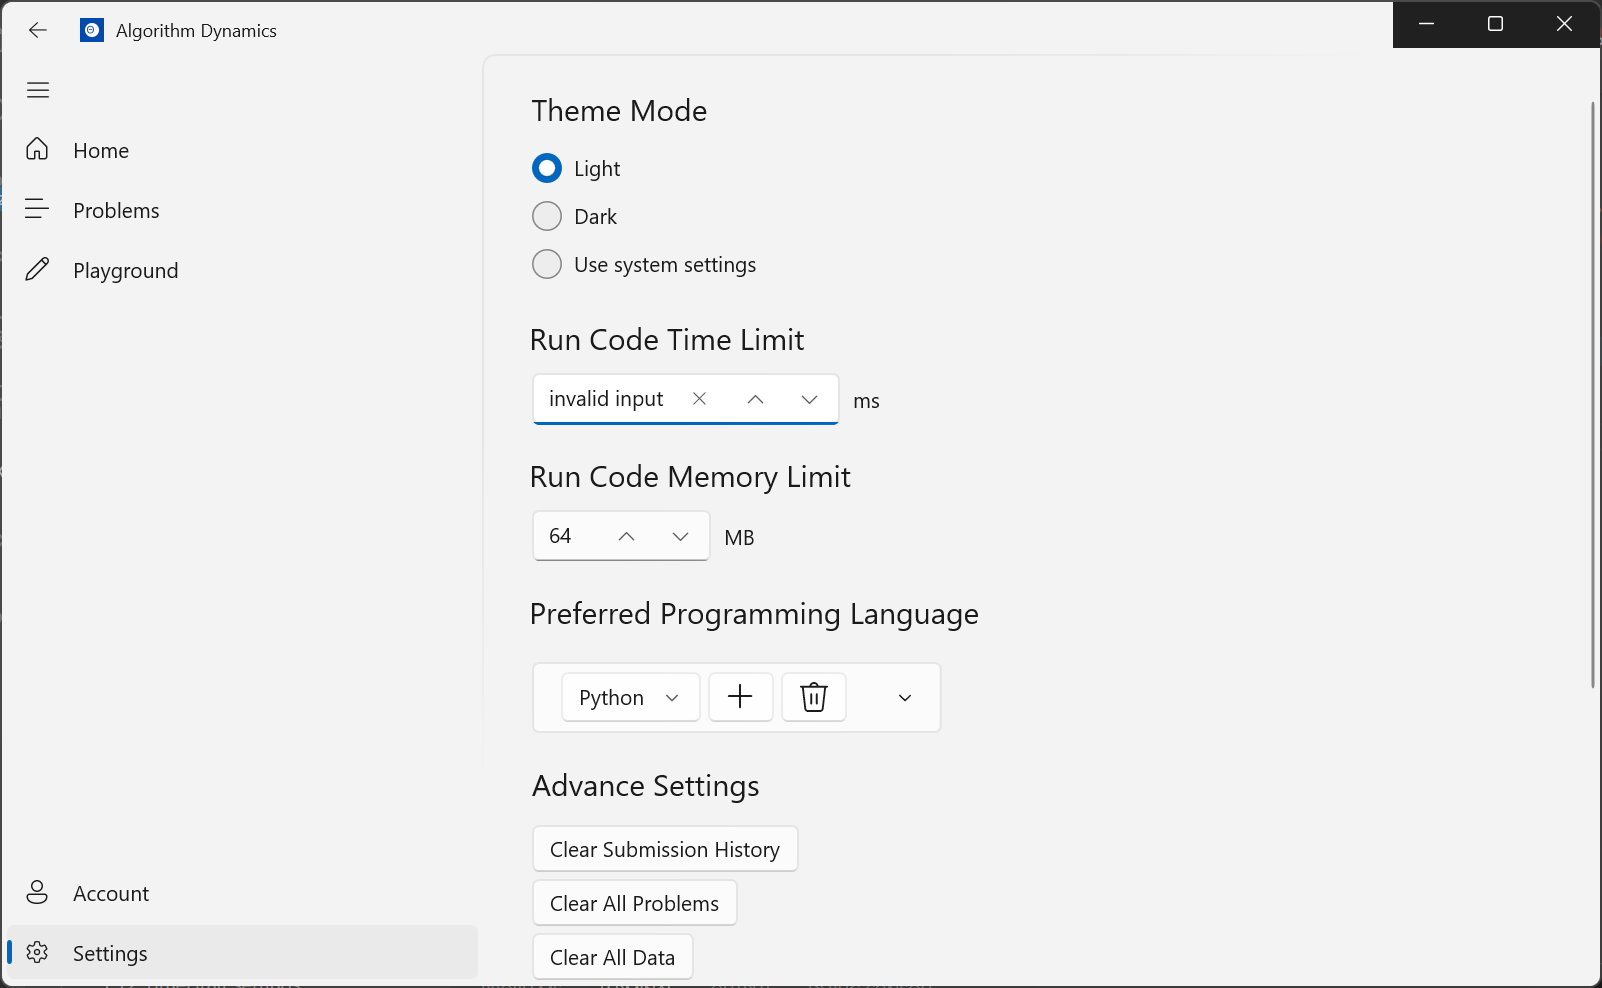
\includegraphics[width=\textwidth, height=\textheight, keepaspectratio]{SettingsPage-TimeLimit-InvalidInput}

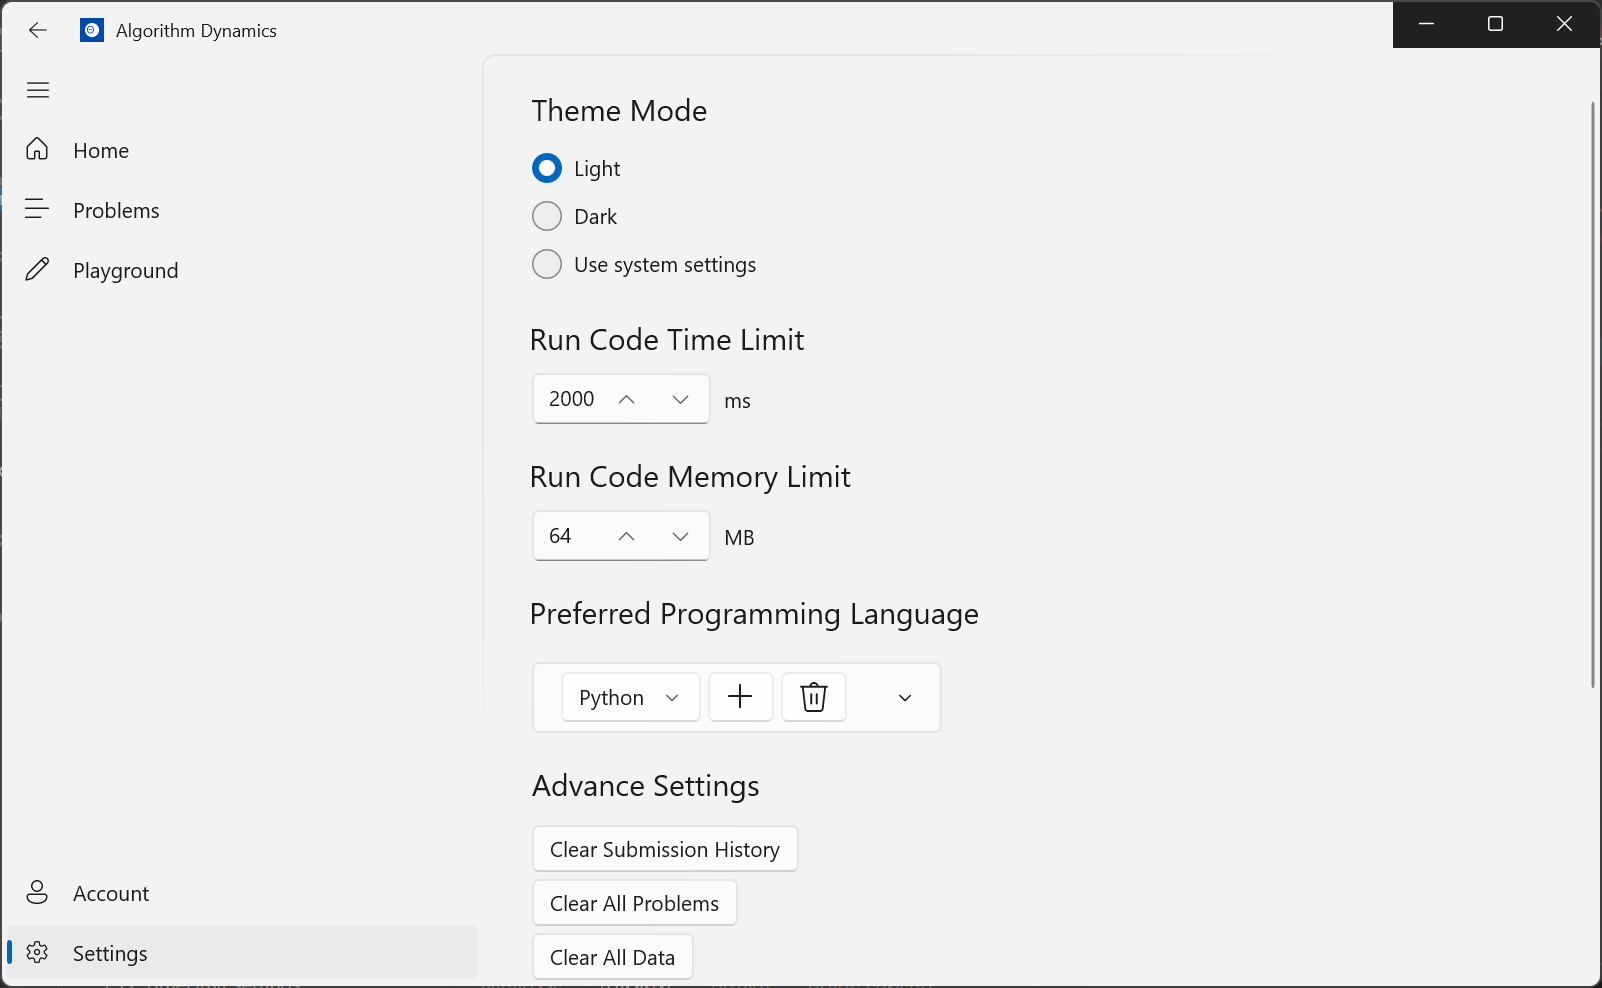
\includegraphics[width=\textwidth, height=\textheight, keepaspectratio]{SettingsPage-TimeLimit-Save}

In the PlaygroundPage, the value for the TimeLimit setting is read and applied.

\begin{minted}{csharp}
/// <summary>
/// RunCode using <see cref="Judger.RunCode"/>
/// </summary>
/// <param name="sender"></param>
/// <param name="e"></param>
private async void RunCodeButton_Click(object sender, RoutedEventArgs e)
{
    ApplicationDataContainer localSettings 
        = ApplicationData.Current.LocalSettings;
    // Read RunCode TimeLimit from settings
    var CurrentTimeLimit = localSettings.Values[TIMELIMIT_KEY];
    if (CurrentTimeLimit != null)
    {
        _timeLimit = (int)CurrentTimeLimit;
    }
    else
    {
        localSettings.Values[TIMELIMIT_KEY] 
            = DEFAULT_RUN_CODE_TIMELIMIT;
    }

    // ... RunCode logic
}
\end{minted}

The process is killed after 2000ms in the PlaygroundPage.

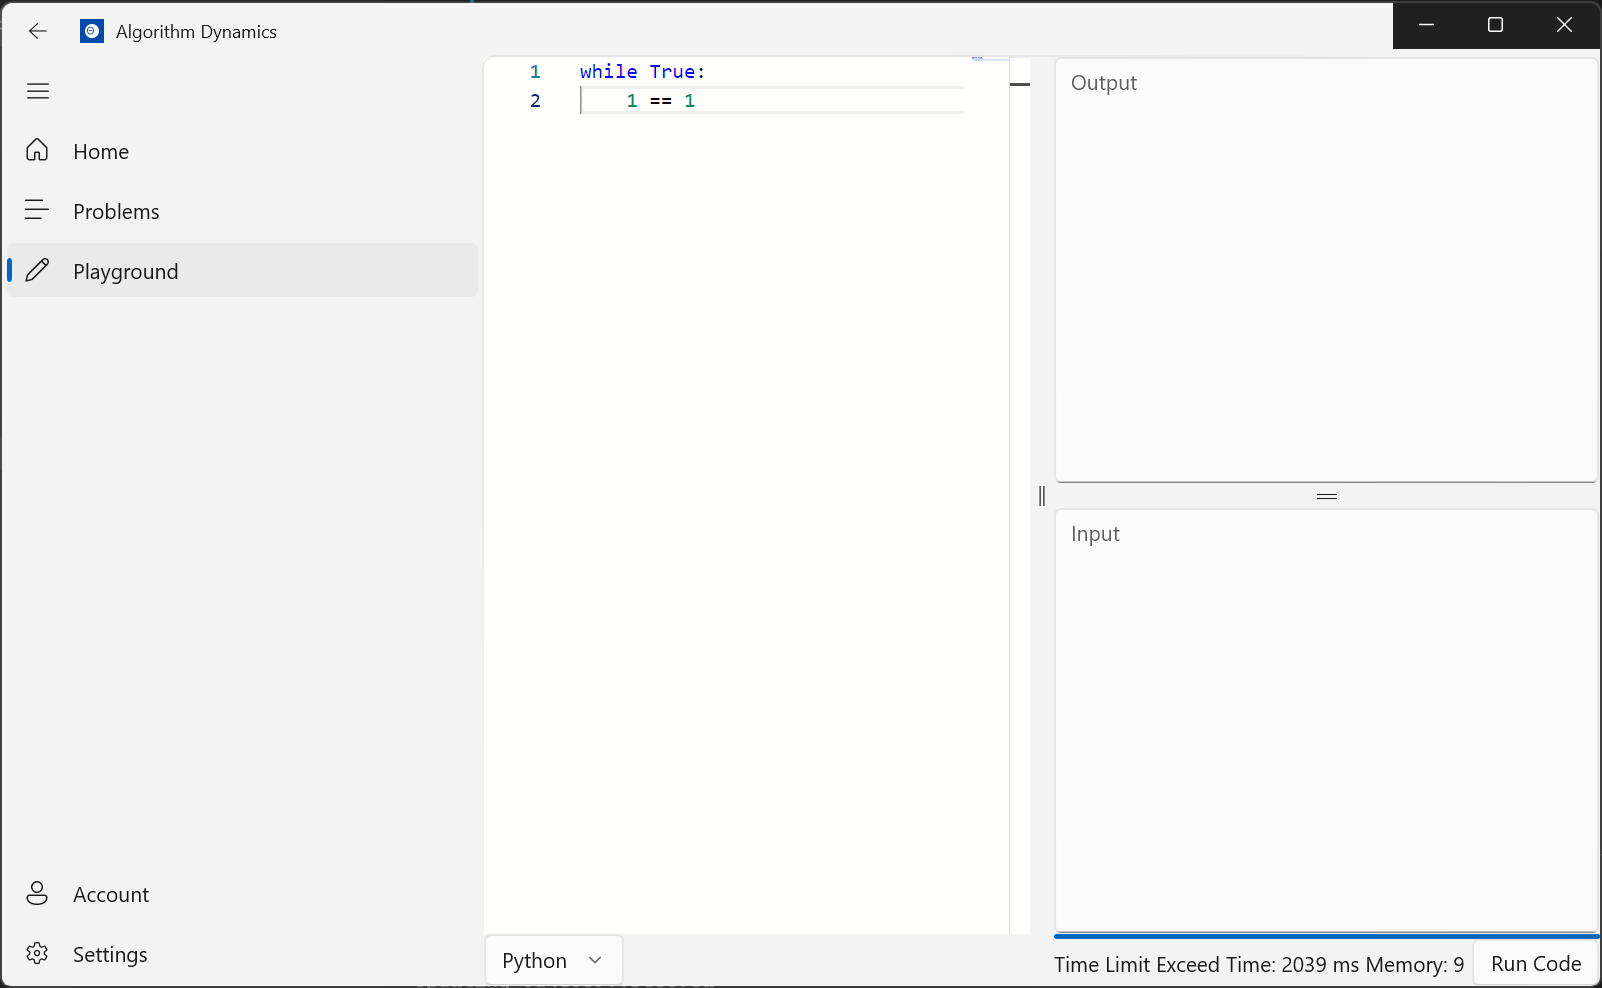
\includegraphics[width=\textwidth, height=\textheight, keepaspectratio]{PlaygroundPage-RunCodeTimeLimit}

\subsection{MemoryLimit settings}

Similar to the TimeLimit setting, I first add \code{MemoryLimit} to the SettingsPage.

\begin{minted}{csharp}
/// <summary>
/// The RunCode MemoryLimit value
/// </summary>
public int MemoryLimit
{
    get
    {
        // Read memory limit from settings
        // If does not exist, store the default memory limit
        ApplicationDataContainer localSettings = ApplicationData.Current.LocalSettings;
        var CurrentValue = localSettings.Values[MEMORYLIMIT_KEY];
        if (CurrentValue != null)
        {
            return (int)CurrentValue / MB;
        }
        else
        {
            localSettings.Values[MEMORYLIMIT_KEY] = DEFAULT_RUN_CODE_MEMORYLIMIT;
            return DEFAULT_RUN_CODE_MEMORYLIMIT / MB;
        }
    }
    set
    {
        // Update the setting
        ApplicationDataContainer localSettings = ApplicationData.Current.LocalSettings;
        localSettings.Values[MEMORYLIMIT_KEY] = value * MB;
    }
}
\end{minted}

Then load it from the PlaygroundPage.

\begin{minted}{csharp}
// Read RunCode MemoryLimit from settings
var CurrentMemoryLimit = localSettings.Values[MEMORYLIMIT_KEY];
if (CurrentMemoryLimit != null)
{
    _memoryLimit = (int)CurrentMemoryLimit;
}
else
{
    localSettings.Values[MEMORYLIMIT_KEY] 
        = DEFAULT_RUN_CODE_MEMORYLIMIT;
}

// Run Code
RunCodeResult result = await Judger.RunCode(
    CodeEditor.Code,
    Input,
    Languages[LanguageComboBox.SelectedIndex],
    _timeLimit,
    _memoryLimit,
    progress);
\end{minted}

The process is killed after exceeding 32 MB of memory usage, which means the memory limit setting is working correctly.

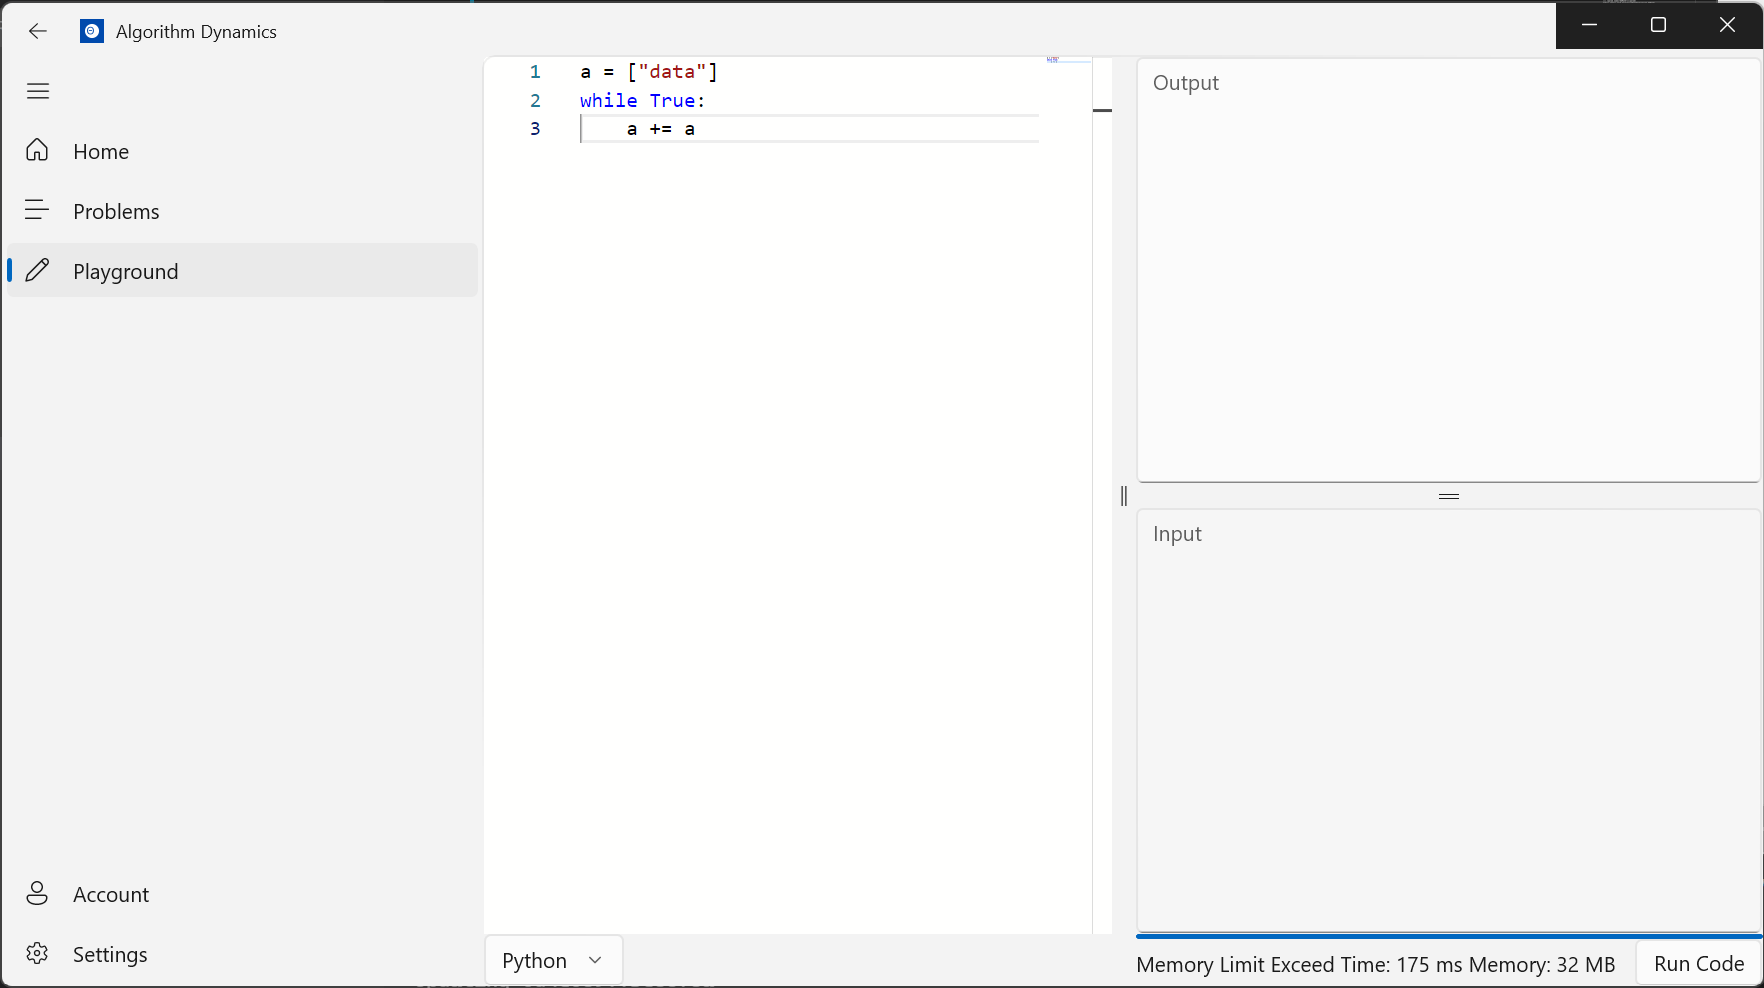
\includegraphics[width=\textwidth, height=\textheight, keepaspectratio]{PlaygroundPage-RunCodeMemoryLimit}

\subsection{Current User settings}

The settings also store an item that cannot be edited directly, the current user id. All user data is stored in the database, the current user id in the settings determines what gets recorded to the code submissions record and the greeting message on HomePage.

In App.xaml.cs, I created a global method to get the current id, so it can be used easily anywhere in the app.

\begin{minted}{csharp}
/// <summary>
/// Get the current user.
/// </summary>
public static User CurrentUser
{
    get
    {
        ApplicationDataContainer localSettings = ApplicationData.Current.LocalSettings;
        Guid uid = (Guid)localSettings.Values["CurrentUser"];
        return User.Get(uid);
    }
}
\end{minted}

In HomePage.xaml.cs, I get the current user name and display it on the screen.

\begin{minted}{csharp}
private void SetWelcomeMessage()
{
    // Get current user name
    string userName = "User";
    if (App.CurrentUser != null)
    {
        userName = App.CurrentUser.Name;
    }

    // Set WelcomeMessage
}
\end{minted}

The current user value is only set on the first startup. When creating the user on the welcome page, the user id should also be stored in the settings.

\begin{minted}{csharp}
/// <summary>
/// Create a new user and store <see cref="User.Uid"/> into settings
/// </summary>
/// <param name="sender"></param>
/// <param name="e"></param>
private void CreateUserButton_Click(object sender, RoutedEventArgs e)
{
    // Create user
    User user = User.Create(UserName, Email, Role);

    // Set current user
    ApplicationDataContainer localSettings = ApplicationData.Current.LocalSettings;
    localSettings.Values["CurrentUser"] = user.Uid;

    // Navigate to HomePage
    WelcomeGrid.Visibility = Visibility.Collapsed;
    MainNavView.SelectedItem = MainNavView.MenuItems[0];
}
\end{minted}

Hence, all functions related to the local settings are implemented and tested.

\subsection{Stakeholder feedback}

The stakeholders are very satisfied with all the settings options and how they can be changed and loaded seamlessly.

\end{document}